% 2010 年江西卷理科第 20 题：两个共边正三角形 BCD、MCD 与垂线段 AB。
% 来源 PDF：普通高考/2010/2010江西理.pdf，SHA-256 994a56c33da151e22af3fabe292d1b5b193866dfc35773a4431e6dfc8a0cc934。
% 原页：第 2 页（A3 三栏）第 1 栏中部，书页码 608。
% 重绘依据：照原页视角，A 在 B 正上方（AB⊥底面），C 在下，D 在右，M 在 CD 中点的正上方
%   （平面 MCD⊥平面 BCD）；可见棱 AB、AC、AD、AM、BC、CD、MC、MD 画实线，BD、BM 画虚线。
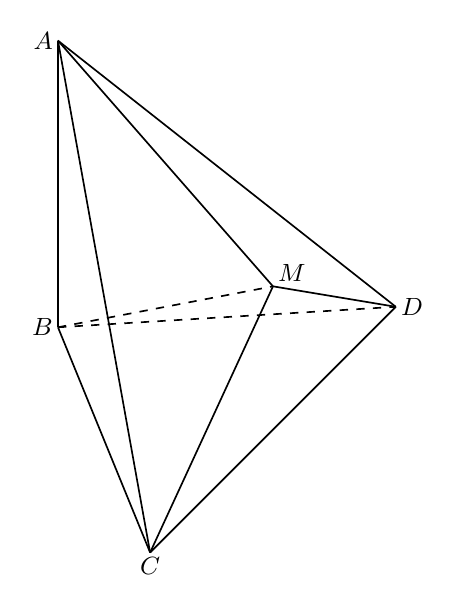
\begin{tikzpicture}[semithick, scale=1.3, every node/.style={inner sep=1.6pt, font=\small}]
  \coordinate (B) at (0,0);
  \coordinate (A) at (0,2.8);
  \coordinate (C) at (0.9,-2.2);
  \coordinate (D) at (3.3,0.2);
  \coordinate (M) at (2.1,0.4);
  \draw (A) -- (B);
  \draw (A) -- (C);
  \draw (A) -- (D);
  \draw (A) -- (M);
  \draw (B) -- (C);
  \draw (C) -- (D);
  \draw (M) -- (C);
  \draw (M) -- (D);
  \draw[dashed] (B) -- (D);
  \draw[dashed] (B) -- (M);
  \node[left] at (A) {$A$};
  \node[left] at (B) {$B$};
  \node[below] at (C) {$C$};
  \node[right] at (D) {$D$};
  \node[above right] at (M) {$M$};
\end{tikzpicture}
